\documentclass[11pt]{article}
\usepackage{mathpicture}

\begin{document}
\begin{figure}[htb]
    \centering
    \subfigure[(第10题)]{
    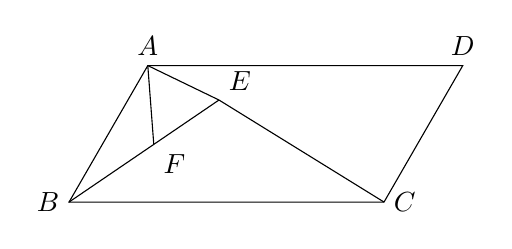
\begin{tikzpicture}[scale=0.4]
        \coordinate[label=above:{$A$}] (A) at (2.5,4.33333);
        \coordinate[label=left:{$B$}] (B) at (0,0);
        \coordinate[label=above:{$D$}] (D) at (12.5,4.33333);
        \coordinate[label=right:{$C$}] (C) at (10,0);
        \coordinate[label=above right:{$E$}] (E) at (4.76,3.24);
        \coordinate[label=below right:{$F$}] (F) at (2.69,1.83);
        \draw (A) -- (B) -- (C) -- (D) -- cycle;
        \draw (A)--(F);
        \draw (A)--(E);
        \draw (C)--(E);
        \draw (B)--(E);
    \end{tikzpicture}}
\end{figure}
\end{document}